\documentclass[tikz, border=10pt]{standalone}
\usetikzlibrary{shapes,fit}

\tikzset{
    pics/vhsplit/.style n args = {6}{
        code = {
        \draw [draw] (0,1) rectangle (1.25,0.5);
        \node[draw=none] at (0.625,0.75) {#1};
        \draw [draw] (1.25,1) rectangle (2,0.5);
        \node[draw=none] at (1.625,0.75) {#2};
        \draw [draw] (0,0.5) rectangle (0.5,0);
        \draw [draw] (0.5,0.5) rectangle (1,0);
        \draw [draw] (1,0.5) rectangle (1.5,0);
        \draw [draw] (1.5,0.5) rectangle (2,0);
        \node[draw=none] at (0.25,0.25) {\tiny{#3}};
        \node[draw=none] at (0.75,0.25) {\tiny{#4}};
        \node[draw=none] at (1.25,0.25) {\tiny{#5}};
        \node[draw=none] at (1.75,0.25) {\tiny{#6}};
        }
    }
}


\begin{document}
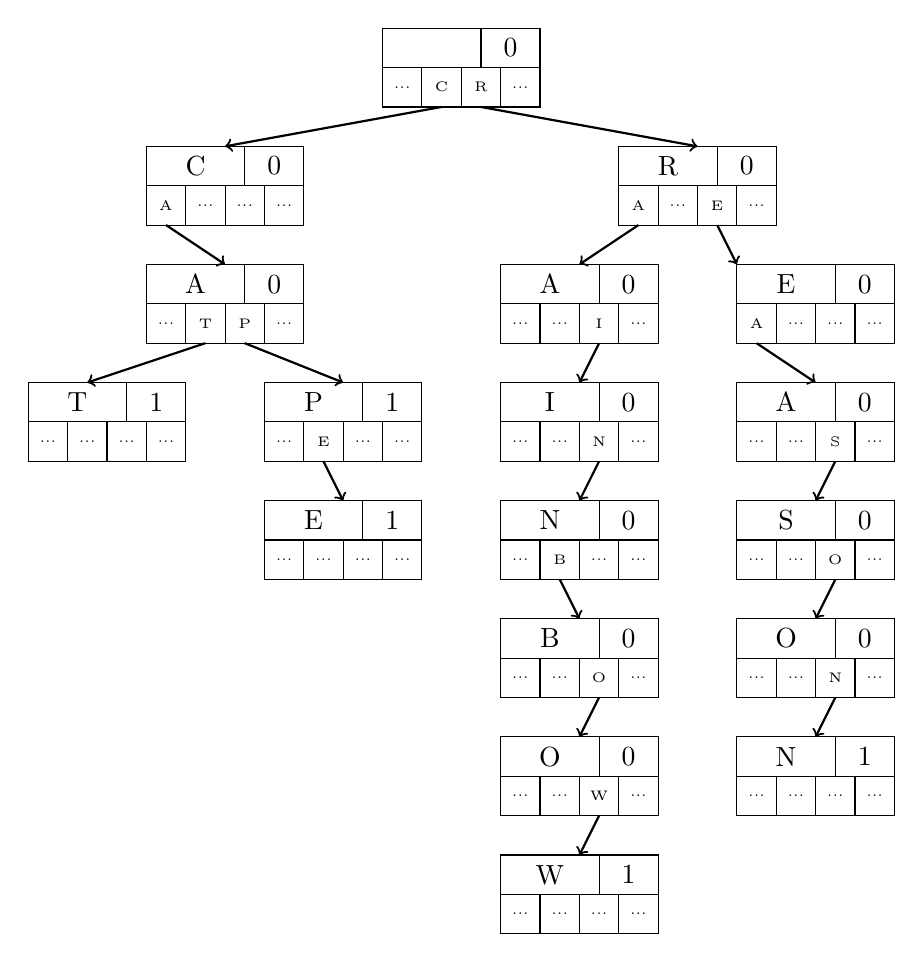
\begin{tikzpicture}%[every node/.append style={draw, rounded corners, inner sep=10pt}]
    \path pic {vhsplit={}{0}{...}{C}{R}{...}};
    \coordinate(Cs) at (0.75,0);
    \coordinate(Rs) at (1.25,0);

    \path pic at (-3,-1.5) {vhsplit={C}{0}{A}{...}{...}{...}};
    \coordinate(Cn) at (-2,-0.5);
    \coordinate(As) at (-2.75,-1.5);

    \path pic at (-3,-3) {vhsplit={A}{0}{...}{T}{P}{...}};
    \coordinate(An) at (-2,-2);
    \coordinate(Ts) at (-2.25,-3);
    \coordinate(Ps) at (-1.75,-3);

    \path pic at (-4.5,-4.5) {vhsplit={T}{1}{...}{...}{...}{...}};
    \coordinate(Tn) at (-3.75,-3.5);

    \path pic at (-1.5,-4.5) {vhsplit={P}{1}{...}{E}{...}{...}};
    \coordinate(Pn) at (-0.5,-3.5);
    \coordinate(Es) at (-0.75,-4.5);

    \path pic (E) at (-1.5,-6) {vhsplit={E}{1}{...}{...}{...}{...}};
    \coordinate(En) at (-0.5,-5);

    \draw [->,  thick] (Cs)--(Cn);
    \draw [->,  thick] (As)--(An);
    \draw [->,  thick] (Ts)--(Tn);
    \draw [->,  thick] (Ps)--(Pn);
    \draw [->,  thick] (Es)--(En);

    \path pic at (3,-1.5) {vhsplit={R}{0}{A}{...}{E}{...}};
    \coordinate(Rn) at (4,-0.5);
    \coordinate(A1s) at (3.25,-1.5);
    \coordinate(E1s) at (4.25,-1.5);

    \path pic at (1.5,-3) {vhsplit={A}{0}{...}{...}{I}{...}};
    \coordinate(A1n) at (2.5,-2);
    \coordinate(Is) at (2.75,-3);

    \path pic at (4.5,-3) {vhsplit={E}{0}{A}{...}{...}{...}};
    \coordinate(E1n) at (4.5,-2);
    \coordinate(A2s) at (4.75,-3);

    \draw [->,  thick] (Rs)--(Rn);
    \draw [->,  thick] (A1s)--(A1n);
    \draw [->,  thick] (E1s)--(E1n);

    \path pic at (1.5,-4.5) {vhsplit={I}{0}{...}{...}{N}{...}};
    \coordinate(In) at (2.5,-3.5);
    \coordinate(Ns) at (2.75,-4.5);

    \path pic at (1.5,-6) {vhsplit={N}{0}{...}{B}{...}{...}};
    \coordinate(Nn) at (2.5,-5);
    \coordinate(Bs) at (2.25,-6);

    \path pic at (1.5,-7.5) {vhsplit={B}{0}{...}{...}{O}{...}};
    \coordinate(Bn) at (2.5,-6.5);
    \coordinate(Os) at (2.75,-7.5);

    \path pic at (1.5,-9) {vhsplit={O}{0}{...}{...}{W}{...}};
    \coordinate(On) at (2.5,-8);
    \coordinate(Ws) at (2.75,-9);

    \path pic at (1.5,-10.5) {vhsplit={W}{1}{...}{...}{...}{...}};
    \coordinate(Wn) at (2.5,-9.5);

    \draw [->,  thick] (Is)--(In);
    \draw [->,  thick] (Ns)--(Nn);
    \draw [->,  thick] (Bs)--(Bn);
    \draw [->,  thick] (Os)--(On);
    \draw [->,  thick] (Ws)--(Wn);

    \path pic at (4.5,-4.5) {vhsplit={A}{0}{...}{...}{S}{...}};
    \coordinate(A2n) at (5.5,-3.5);
    \coordinate(Ss) at (5.75,-4.5);

    \path pic at (4.5,-6) {vhsplit={S}{0}{...}{...}{O}{...}};
    \coordinate(Sn) at (5.5,-5);
    \coordinate(O1s) at (5.75,-6);

    \path pic at (4.5,-7.5) {vhsplit={O}{0}{...}{...}{N}{...}};
    \coordinate(O1n) at (5.5,-6.5);
    \coordinate(N1s) at (5.75,-7.5);

    \path pic at (4.5,-9) {vhsplit={N}{1}{...}{...}{...}{...}};
    \coordinate(N1n) at (5.5,-8);

    \draw [->,  thick] (A2s)--(A2n);
    \draw [->,  thick] (Ss)--(Sn);
    \draw [->,  thick] (O1s)--(O1n);
    \draw [->,  thick] (N1s)--(N1n);

\end{tikzpicture}
\end{document}
